%%%%%%%%%%%%%%%%%%%%%%%%%%%%%%%%%%%%%%%%%%%%%%%%%%%%%%%%%%%%%%%%%%%%%%%%%%%%%%%%%%%%%%%%%%
\section{Implementation}
%%%%%%%%%%%%%%%%%%%%%%%%%%%%%%%%%%%%%%%%%%%%%%%%%%%%%%%%%%%%%%%%%%%%%%%%%%%%%%%%%%%%%%%%%%i

%
We implemented our \sys prototype in \note{XXX} lines of Rust.
%
We also provide an API server that exposes a JSON-HTTP API that applications
can use to invoke \sys.
%
In the following, we discuss key implementation details that \sys relies for
security and performance.
%

\subsection{Secure Record Storage}
%
An application hands \sys database diffs and speaks-for records when it applies
a disguise $d$.
%
Prior to encrypting these records, \sys appends a random nonce to the plaintext
to prevent known-plaintext attacks.
%
Encryption ensures that only a client with $p$'s private key can reveal these
records.
%

%
\sys must store encrypted records without leaking that disguise $d$ applied to
principal $p$.
%
For example, if \sys revealed that a principal has invoked GDPR deletion, it
might violate the GDPR.
%
Consequently, \sys must avoid storing any mapping from $p$ or $d$ to a bag of
encrypted records, as must the application.
%
However, \sys must also be able to---given $p$, $d$, and $p$'s private
key---decrypt and return records to the application when it invokes
\fn{DiffsForDisguise} or \fn{PseudoprincipalsOf}.
%
While \sys could attempt to decrypt \emph{all} encrypted records with $p$'s
private key, this is clearly too slow for applications with a large amount
of data in \sys.
%
But the client can help the application (and, thus, \sys) identify the bag
of encrypted records for $(p, d)$.
%
This is the role of \sys's locators: each \lcapa{pd} points to a bag of
encrypted records, and \sys maintains an index from locators to bags,
but---crucially---forgets which $(p, d)$ produced the locator.
%

%%%%%%%%%%%%%%%%%%%%%%%%%%%%%%%%%%%%%%%%%%%%%%%%%%%%%%%%%%%%%%
\subsection{Recursive Disguising: Disguising Pseudoprincipals}
\label{s:composition}

\begin{figure}[t]
    \centering
    %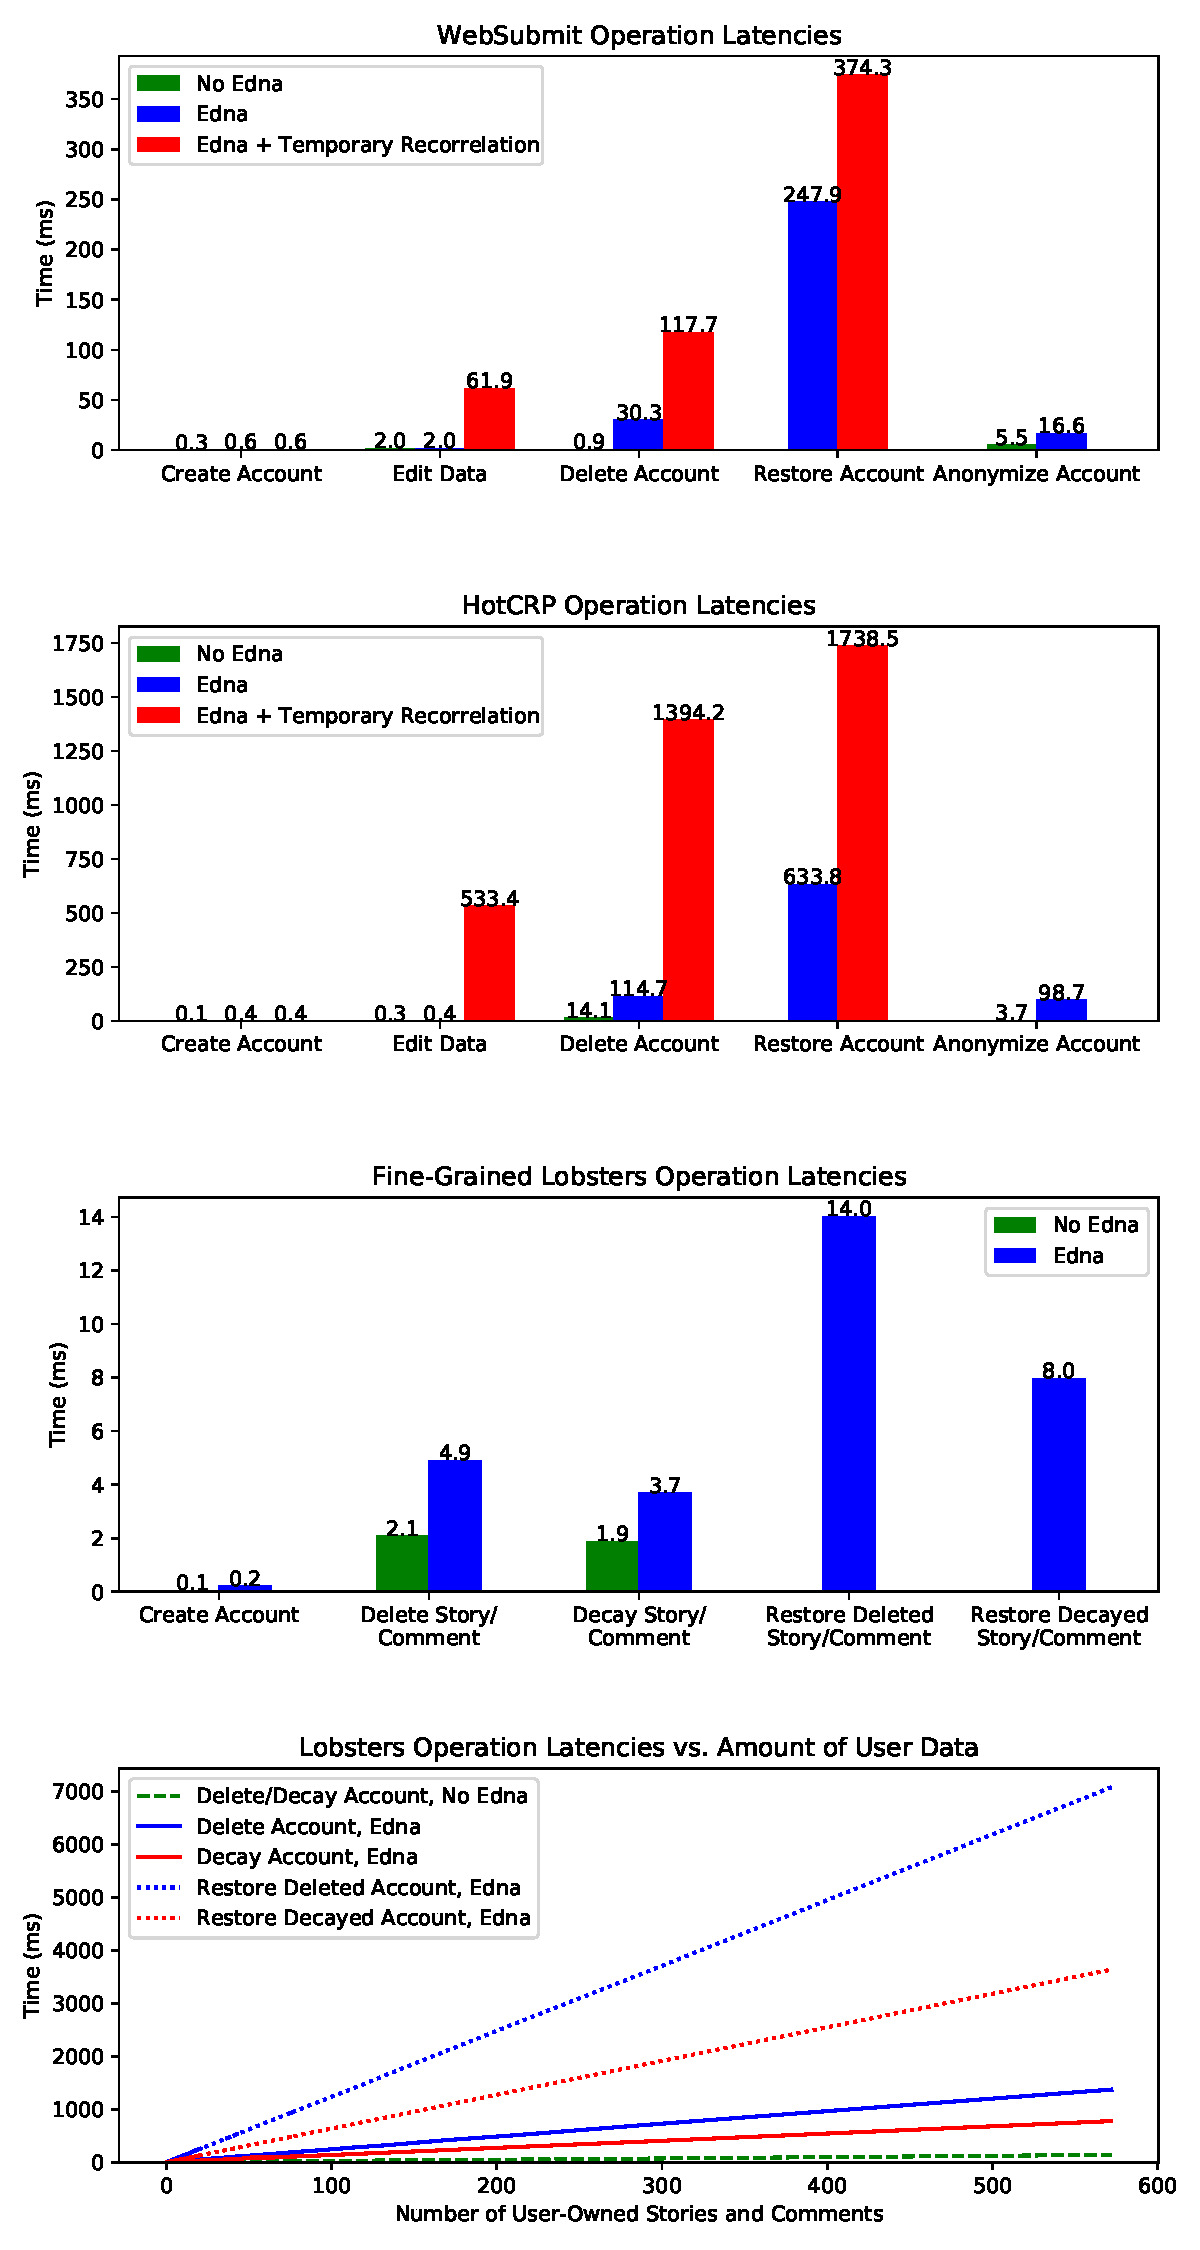
\includegraphics[width=0.5\textwidth]{figs/client_op_stats}
    \caption{Accessing recursively disguised pseudoprincipal records.}
    \label{f:recursive}
\end{figure}

\sys should support disguises that transform data belonging to pseudoprincipals and thus produce
records for pseudoprincipals. For example, pseudoprincipals own every answers after the WebSubmit
admin applies class anonymization. If WebSubmit then performs account deletion of these anonymized
answers, the corresponding answer-removal diff record would be associated with pseudoprincipals.

One might argue that the WebSubmit could associate the answer-removal diff with the original natural
principal owning the answer. However, \sys stll needs to allow disguises to be applied to the data
of pseudoprincipals \emph{even without} knowing the original natural principal who owned the data.
For example, application disguises may have mistakes that require additional disguises to remedy:
the WebSubmit admin might later wish to scrub identifying keywords from answers in addition to
anonymizing them.

\head{How does \sys securely encrypt pseudoprincipal locators?}
\sys must store pseudoprincipal-associated records securely such that only a client with natural
principal $p$'s private key can access $p$'s pseudoprincipals' records. The simplest way would be
to use \pubk{p} to encrypt pseudoprincipal $q$'s records; however, \sys may not know which original principal
$p$ links to $q$.
%
Instead, when \sys creates a new pseudoprincipal for $p$, \sys generates a keypair
\pubk{q} and \privk{q} for pseudoprincipal $q$.
Just like with natural principals, \sys stores \pubk{q} and uses it to encrypt $q$'s records.

\sys then stores \privk{q} such that access to \privk{q} and thus also $q$'s records requires
\privk{p} by
\begin{enumerate}[nosep]
    \item encrypting \privk{q} with \pubk{p} to produce $\enc(\pubk{p}, \privk{q})$, and
    \item storing $\enc(\pubk{p}, \privk{q})$ at location \lcapa{pd} along with $p$'s encrypted diff
records from disguise $d$.
\end{enumerate}

Because of the recursive nature of disguises, $p$ itself may be a pseudoprincipal and not a natural
principal! Thus, the application cannot simply send \privk{q} via \eg email to principal $p$ when it
creates a pseudoprincipal $q$ for $p$.

Generating a single private-public keypair is prohibitively expensive (requiring over 300ms). To
make pseudoprincipal creation---a common operation in disguising---cheap, \sys maintains a
fixed-size pool of pregenerated keys that is periodically refreshed offline. The application tells
\sys an appropriate size of the pool (\eg WebSubmit can estimate the maximum number of users in any
single class, and multiply this by the maximum number of answers each user can submit).

\head{What does \sys do with pseudoprincipal locators?}
\sys stores $q$'s encrypted records from disguise $d$ at some locator \lcapa{qd}.  However, we again
observe that the application and \sys cannot send \lcapa{qd} to some email address when $q$ is a
pseudoprincipal! Instead, \sys saves \lcapa{qd} as part of $q$'s metadata (which also contains $\pubk{q}$).

%To protect pseudoprincipal locators \lcapa{qd}, \sys encrypts \lcapa{qd} with the
%pseudoprincipal's public key \pubk{q} and stores $\enc(\pubk{q}, \lcapa{qd}$) in \sys's metadata for $q$ (which also includes \pubk{q}). This contrasts with how \sys returns locators to the application when storing records for natural principals.

We illustrate in Figure~\ref{f:recursive} how a client that provides private key \privk{p} for
natural principal $p$ and locator \lcapa{pd} may access \emph{both} $p$'s records for disguise $d$
\emph{and} all records of all pseudoprincipals $q$ created during disguise $d$ to decorrelate data
from $p$.  \sys accesses \privk{q} by decrypting \enc(\pubk{p}, \privk{q}) with \privk{p}. With
\privk{q} and \lcapa{qd'} from $q$'s metadata, \sys locates all $q$'s encrypted records,
and then decrypts these records with \privk{q}.
\lyt{TODO clearing of records, $d' \neq d$}

\lyt{Should we note somewhere that pseudoprincipals and recursive disguising are why we need asymmetric
crypto; otherwise, we could just send the symmetric key to the original user being disguised?}

\head{What does \sys do with metadata of deleted pseudoprincipals?}
Recall that \sys removes any metadata (\eg \pubk{p}) about principal $p$ when a disguise removes
$p$'s corresponding principal object.
However, \sys cannot simply remove pseudoprincipal $q$'s metadata when $q$ is removed: this metadata
includes \lcapa{qd} ciphertexts. Removing \lcapa{qd} removes the ability to find $q$'s encrypted
record bags efficiently.
%If \sys wanted to access $q$'s records for \eg disguise reversal, \sys would need
%to attempt to decrypt every encrypted record bag at every location.

Without knowing natural principal-pseudoprincipal correspondences, and thus without any way to send
\lcapa{qd} to a natural principal, \sys has only two choices when $q$ is removed by the application:
(1) delete $q$'s metadata at the cost of losing (efficient) access to $q$'s records, or (2) retain
$q$'s metadata at the cost of slightly weaker security (an adversary learns that a pseudoprincipal
existed and some data had been decorrelated at some point, even if the corresponding user or data
has since been deleted). \sys currently does the latter and retains pseudoprincipal metadata.
%If a pseudoprincipal is often deleted while \sys has knowledge of the link between $q$ and original
%principal $p$ (\eg, when a client deletes $p$'s account and provides speaks-for records
%to \sys to delete $p$'s anoymized data). In these scenarios, \sys can .

%%%%%%%%%%%%%%%%%%%%%%%%%%%%%%%%%%%%%%%%%%%%%%%%%%%%%%%%%%%%%%
\subsection{High-Level Disguise Specifications.}
\sys's high-level disguising API can be used for a restricted set of disguises in applications that
use SQL databases, represent objects as database rows and express principal data ownership via
foreign-key relationships.

Disguises specifications consist of predicated disguise operation specifications and a
pseudoprincipal-generation specification.
\sys performs each operation by selecting database objects that satisfy the predicate; performing SQL queries to modify the objects; and automatically generating and storing records corresponding to the operation performed using \sys's lower-level API.  \sys supports three high-level disguise specification
operations:
\begin{enumerate}[nosep]
    \item Modify: change an attribute of the data object.
    \item Remove: delete the data object.
    \item Decorrelate: generate a pseudoprincipal $q$, and rewrite the foreign key to original
        principal $p$ from the data object to instead point to $q$.
\end{enumerate}
Decorrelation creates a speaks-for record \town{pd} containing the created pseudoprincipal's
ID; removal produces a diff record \tdiff{pd} with the removed object's value; and modification
produces a diff record \tdiff{pd} containing the old and new values of the modified object.

Pseudoprincipal generation specifications consist of a list of per-column policies that each
include the column name, and the selected policy on how to generate values for that column.
\sys supports policies to set values as constants, or to generate random and/or unique strings, emails, past timestamps, phone
numbers, and numbers (in a range).

When revealing disguise $d$, \sys retrieves all records accessible with the provided decryption capability
and locator, and restores the undisguised state by updating the relevant object rows in the database.
To prevent accidental revealing of data that has been updated since $d$ was applied,
\sys will first check that the data to restore is still in its disguised state. If the state of data does
not match the recorded disguised state, then \sys knows the record corresponds to a stale and
overwritten update, and will refuse to restore the undisguised state.

%%%%%%%%%%%%%%%%%%%%%%%%%%%%%%%%%%%%%%%%%%%%%%%%%%%%%%%%%%%%%%

\iffalse
\sys enables HotCRP to support the following features:
\begin{itemize}
    \item\emph{1st-Party GDPR-Compliant Disguising:}
HotCRP supports user-invoked disguise(s) to modify, decorrelate and/or delete the user's data and
account, meeting the requirements of the GDPR's right to be forgotten.

    \item \emph{1st-Party Disguised Data Restoration}: HotCRP users who invoke GDPR deletion are given the
        option to return by revealing their disguise; however, between disguising and revealing
        their account, no other entity learns the identity or existence of the user (ensuring that
        the disguise complies with the GDPR).

    \item\emph{3rd-Party Disguising.}
\sys supports disguises applied by users (such as an admin) that transform data of other users in the system. For example, universal conference anonymization or
    comment removal alters data not associated with the invoking admin.

\item \emph{Data Decay}: After several years, the admin can decay identifiers in the conference data
    by decorrelating all users from their authored reviews and papers.  This helps protect reviewers
        and paper authors from being unblinded in the case of a data breach.

\item \emph{Temporary Recorrelation with Anonymized Data}:
Even after universal decorrelation, HotCRP allows users to apply GDPR account
deletion to delete even their decorrelated papers and reviews that they wrote.
%

%
Furthermore, HotCRP users can also view reviews on their papers, or edit their reviews, even if
        these papers and reviews have been decorrelated and belong to anonymous users.  HotCRP users
        interact with a personalized, temporary database view when they visit their decorrelated
        data.

Data disguising enables temporary recorrelation to support these use cases \emph{without} changing
        the database contents and revealing to other users of the system
which actual user authored these anonymized papers and reviews.

\item \emph{Further Disguising of Anonymized Users' Data}: A disguise such as universal comment
        removal can be applied after universal decorrelation, even though it now applies to data of anonymous users.
This allows disguises to be developed over time, and to remove identifying data potentially mistakenly missed by prior
disguises, but which now belongs to anonymous users.
\end{itemize}
\fi
